\documentclass[10pt,A4]{article}

%set margin
\usepackage[a4paper]{geometry}		
\geometry{top=1cm, bottom=-.6cm, left=0.4cm, right=1cm} 

\usepackage{graphicx}
\graphicspath{ {./} }

\newcommand\tab[1][1cm]{\hspace*{#1}}

%for cell's color of table
\usepackage{xcolor,colortbl}

%star rating system
\usepackage{tikz}
\usetikzlibrary{shapes.geometric}
\newcommand\score[2]{
\pgfmathsetmacro\pgfxa{#1+1}
\tikzstyle{scorestars}=[star, star points=5, star point ratio=2.25, draw, inner sep=1.3pt, anchor=outer point 3]
  \begin{tikzpicture}[baseline]
    \foreach \i in {1,...,#2} {
    \pgfmathparse{(\i<=#1?"yellow":"white")}
    \edef\starcolor{\pgfmathresult}
    \draw (\i*1.75ex,0) node[name=star\i,scorestars,fill=\starcolor]  {};
   }
  \end{tikzpicture}
}



\usepackage[most]{tcolorbox}
\newtcbtheorem{Summary}{\bfseries Skills}{enhanced,drop shadow={black!50!white},
  coltitle=black,
  top=0.3in,
  attach boxed title to top right=
  {xshift=0em,yshift=-\tcboxedtitleheight/2},
  boxed title style={size=small,colback=pink}
}{summary}

\usepackage{multicol}

\usepackage[utf8x]{inputenc}
\usepackage{tikz}
\usepackage{varwidth}
\usepackage{linegoal}
\usepackage[explicit]{titlesec}
\usepackage[margin=1.5cm]{geometry}

\titleformat{name=\section,numberless}
  {\normalfont\Large\bfseries}{}{0em}
  {%
  \begin{tikzpicture}
  \node[inner xsep=0pt,text width=\textwidth,
    align=left,left color=myblue,right color=myblue!10] 
    {\parbox[t]{\linewidth}{\raggedright#1}};
  \end{tikzpicture}%
  }



\begin{document}
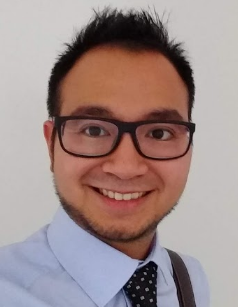
\includegraphics[width=30mm]{myphoto}
\begin{quotation}
" Expert in Administrating of DevOps and Linux system, I am looking forward to exploiting my skills in a new domaine."
\end{quotation}

\begin{minipage}[c]{0.7\textwidth}
%---------------------------------------------------------------------------------------
%	EXPERIENCE
%----------------------------------------------------------------------------------------

\section*{A test unnumbered section with a really long title spanning several lines just for the example}

\section*{\noindent\colorbox{cyan!20}{\makebox[\dimexpr\linewidth-2\fboxsep\relax][l]{Experience}}}

\subsubsection*{2019 - now : Linux and DevOps PaaS Administrator - Capgemini Toulouse}
\begin{itemize}
  \item Develop the DevOps Platform as a Service on premise
  \item Develop the Proof of Concept Demonstrator for DevOps on diffrent technologies    
  \item Redact the DevOps guide and best pratices
  \item Provide support on migration from old school to DevOps
  \item Provide support to end-users on traditional Linux Platform
\end{itemize}

\subsubsection*{2013 - 2018 : Thermal Software Development Engineer / Thermal Simulation Engineer - Altran Technologies Toulouse}
\begin{itemize}
  \item Invented a flexible assessment framework, targeting industrial trainees
  \item TOICA
  \item Build numerical model and Performed thermal simultion to certificate the design of Aircraft (global model A350-900 , pre-cooler A320 NEO), electronic cards
  \item Supervised internships on thermal software development, Recruited trainees
\end{itemize}

\subsubsection*{2012 -2013 : Aerodynamics Software Developement Engineer - Altran Technologies}
\begin{itemize}
  \item Tool migration from Fortran to Python
  \item Provided suport for Aero - Simulation platform and tools
\end{itemize}

%--------------------------------------------------------------------------------------
%	EDUCATION SECTION
%--------------------------------------------------------------------------------------

\section*{\noindent\colorbox{cyan}{\makebox[\dimexpr\linewidth-2\fboxsep\relax][l]{Diplome \& Certificates}}}

\subsubsection*{2011 : Graduated as M.Sc. Digital Media - University of Bremen}
Master Thesis: Semi Automated Scoring in Technology Based Assessment



\section*{\noindent\colorbox{cyan}{\makebox[\dimexpr\linewidth-2\fboxsep\relax][l]{Others}}}

\begin{itemize}
  \item Conceive an DevOps airgap PaaS basing on Kubernetes solution with Rancher as an UI
  \item Define the DevOps best pratices
  \item Migrate applications to the new PaaS
\end{itemize}

\section*{\colorbox{red}{Example 1}}\index{Paragraphs of Text}
\section*{\noindent\colorbox{cyan}{\makebox[\dimexpr\linewidth-2\fboxsep\relax][l]{Others}}}

{\noindent\colorbox{cyan}{\makebox[\dimexpr\linewidth-2\fboxsep\relax][l]{test}}}

test

{\noindent\hspace*{\dimexpr-\oddsidemargin-1in\relax}%
 \colorbox{cyan}{\makebox[\dimexpr\paperwidth-2\fboxsep\relax]{test}}%
 \hspace*{-\paperwidth}}
\end{minipage}
\begin{minipage}[t]{0.05\textwidth}
\end{minipage}
\begin{minipage}[c]{0.25\textwidth}
\begin{comment}
\begin{tcolorbox}[enhanced,width=2.5in,center upper,size=fbox,
    fontupper=\large\bfseries,drop shadow southwest,sharp corners]

\begin{center}
{\noindent\colorbox{cyan}{\makebox[\dimexpr\linewidth-2\fboxsep\relax]{
\textless competences/\textgreater
}}}
\end{center}
\end{comment}
\begin{tabular}{|lc|}
\hline
\multicolumn{2}{|c|}{\cellcolor{white}Web App Development} \\
\hline
Angular & \score{3}{5} \\
Djanggo & \score{2}{5} \\
HTML & \score{4}{5} \\
CSS & \score{4}{5} \\
Python & \score{5}{5} \\
Node.js & \score{3}{5} \\
\hline
\multicolumn{2}{c}{} \\
\hline
\multicolumn{2}{|c|}{\cellcolor{white}DevOps Culture} \\
\hline
Git & \score{5}{5} \\
Jenkins & \score{5}{5} \\
Artifactory & \score{5}{5} \\
Ansible & \score{3}{5} \\
\hline
\multicolumn{2}{c}{} \\
\hline
\multicolumn{2}{|c|}{\cellcolor{white}DevOps Infrastructure} \\
\hline
Docker & \score{5}{5} \\
Kubernetes & \score{4}{5} \\
Rancher & \score{5}{5} \\
Helm & \score{4}{5} \\
AWS & \score{3}{5} \\
Openshift & \score{2}{5} \\
\hline
\end{tabular}

%\end{tcolorbox}

\end{minipage}

\end{document}
